%% Latex instantiation based on template for PhD dissertation or MS thesis
%% Brigham Young University

\documentclass[12pt]{report}

%%%%%%%%%%%%%%%%%%%%%%%%%%%%%%%%%%%%%%%%%%%%%%%%%%%%%%%%
%  Setup BYU thesis format
%%%%%%%%%%%%%%%%%%%%%%%%%%%%%%%%%%%%%%%%%%%%%%%%%%%%%%%%%
\usepackage{byustyle}
% Setup the byu style sheet
\byustylesetup{%
    %
    %isdissertation = true,            % Uncomment this if you're doing a PhD dissertation
    %etdsubmission = true,            % Uncomment this if you're compiling it for ETD submission
    singlepageabstract = true, % Comment this out if your abstract is multiple pages
    %singlepageacknowledgements = true, % Uncomment this if your Acknowledgements is multiple pages
    %
    % Definitions of names needed in thesis/dissertation
    deptname          = Department of Humanities,    %
    collegename       = Linguistics, %
    committeechairman = Deryle Lonsdale,                      %
    committeemembera  = Mark Davies,                         %
    committeememberb  = Stephen Liddle,                          %
    %committeememberc  = Firstname Mi. Lastname,                    % PhD Only
    %committeememberd  = Firstname Mi. Lastname,                     % PhD Only
    graddate = June 2016,  % Leave commented for current month and year
    %copyrightyear = 2016,      % Leave commented for current year
    % uncomment the keywords for a dissertation
    keywords         = {LDA, Gibbs Sampling, k-NN, Hellinger Distance, Jenson Shannon Divergence, IR, recommendation systems, text mining, LDS Scripture Citation Index, SCI, RelRec, topic modeling}
    %
    % Uncomment to shorten for proofreading purposes
    %noabstract = true,         % Don't show the abstract page
    %nouniversitypages = true,  % Don't show any of the "university pages"
    %noacknowledgements = true, % Don't show the Acknowledgements page
    %notableofcontents = true,  % Don't show the Table of Contents
    %nolistoffigures = true,    % Don't show the List of Figures
    %nolistoftables = true,     % Don't show the List of Tables
    %notocandlists = true,      % Don't show the Table of Contents, List of Figures, or the List of Tables
    %noheaderatall = true,      % Don't show any of the BYU Thesis header pages
}
%%%%%%%%%%%%%%%%%%%%%%%%%%%%%%%%%%%%%%%%%%%%%%%%%%%%%%%%
%  END:  Setup BYU thesis format
%%%%%%%%%%%%%%%%%%%%%%%%%%%%%%%%%%%%%%%%%%%%%%%%%%%%%%%%%

%%%%%%%%%%%%%%%%%%%%%%%%%%%%%%%%%%%%%%%%%%%%%%%%%%%%%%%%
%  Include other \usepackage{} statements here.
%    Add one package at a time.
%    Warning:  Some packages are not compatible with byuthesis.sty
%%%%%%%%%%%%%%%%%%%%%%%%%%%%%%%%%%%%%%%%%%%%%%%%%%%%%%%%%
%\usepackage[normalmargins]{savetrees} % prints smaller to save trees (draft only)
\usepackage{amsmath,amssymb} % math definitions
\usepackage{graphicx}        % for figures
\usepackage{subfigure}       % for figures with multiple subfigures
\usepackage{setspace}        % so all the captions will be single spaced
%%%%%%%%%%%%%%%%%%%%%%%%%%%%%%%%%%%%%%%%%%%%%%%%%%%%%%%%
%  END: Include other \usepackage{} statements here.
%%%%%%%%%%%%%%%%%%%%%%%%%%%%%%%%%%%%%%%%%%%%%%%%%%%%%%%%%

%%%%%%%%%%%%%%%%%%%%%%%%%%%%%%%%%%%%%%%%%%%%%%%%%%%%%%%%
% For doing bookmarks in the PDF file
%%%%%%%%%%%%%%%%%%%%%%%%%%%%%%%%%%%%%%%%%%%%%%%%%%%%%%%%%
% For more info, see:
% http://www.geocities.com/kijoo2000/latex2pdf.pdf
% http://www.tug.org/applications/hyperref/manual.html
\usepackage[backref,pagebackref,plainpages=false,driverfallback=dvipdfm]{hyperref}
\hypersetup{
    %bookmarks    = true, % Make bookmarks (default=true). This option
                          %cannot be used after package has been loaded,
                          %thus use like this: \usepackage[bookmarks=false]{hyperref}.
    %
    breaklinks   = false, % Allow link text to break across lines (default=false).
    linktocpage  = false, % make page number, not text, be link on TOC, LOF and LOT
    colorlinks   = false, % Color the text of links (true) or put color frames over
                          % the links (false).
% NOTE: if you need to use a dvi->ps->pdf path for things like PSTricks, you
% may find that commenting out the next line is necessary.
    pdfborder    = 001,   % sets the default for pdf links
    pdfstartview = {FitH}, % Set the startup page view. Possible options are:
                           % FitH: Fit whole width of page
                           % FitV: Fit whole height of page
                           % FitB: Fit whole �Bounding Box� page
                           % FitBH: Fit whole width of �Bounding Box� of page
                           % FitBV: Fit whole height of �Bounding Box� of page
    bookmarksnumbered  = true, % Put section numbers in bookmarks (default=false)
    bookmarksopen      = true, % Open up the bookmark trees (default=false).
    bookmarksopenlevel = 1, % Level to which bookmarks are open (default=\maxdimen).
    bookmarkstype      = toc, % Specify which toc file to mimic (default=toc).
    pdfpagemode        = {UseOutlines}, %  Specify how document starts when opened ({None}).
                                        % Possible options are:,
                                        % None: Neither bookmarks nor thumbnails are visible.
                                        % UseOutlines: Bookmarks are visible.
                                        % UseThumbs: Thumbnails are visible.
                                        % FullScreen: Full-screen mode
    pdftitle    = {Mark Davies},
    pdfauthor   = {Michael G. Bean},
    pdfcreator  = {Michael G. Bean},
    pdfsubject  = {Michael G. Bean's Master's Thesis},
    pdfkeywords = {Thesis Template, BYU},
}
%%%%%%%%%%%%%%%%%%%%%%%%%%%%%%%%%%%%%%%%%%%%%%%%%%%%%%%%
%  END: For doing bookmarks in the PDF file
%%%%%%%%%%%%%%%%%%%%%%%%%%%%%%%%%%%%%%%%%%%%%%%%%%%%%%%%%

%%%%%%%%%%%%%%%%%%%%%%%%%%%%%%%%%%%%%%%%%%%%%%%%%%%%%%%%
%                Macros
%  Define macros here
%%%%%%%%%%%%%%%%%%%%%%%%%%%%%%%%%%%%%%%%%%%%%%%%%%%%%%%%%
\def\proof{\noindent{\it Proof: }}
\def\QED{\mbox{\rule[0pt]{1.5ex}{1.5ex}}}
\def\endproof{\hspace*{\fill}~\QED\par\endtrivlist\unskip}
%
\newcommand{\norm}[1]{\left\|#1\right\|}
\newcommand{\abs}[1]{\left|#1\right|}
\newcommand{\defeq}{\stackrel{\triangle}{=}}
\newcommand{\re}{\mathbb{R}} % real numbers
\newcommand{\OMIT}[1]{{}} % omit sections of text
\newcommand{\pd}[2]{\ensuremath{\frac{\partial #1}{\partial #2}}} % partial derivative

%%%%%%%%%%%%%%%%%%%%%%%%%%%%%%%%%%%%%%%%%%%%%%%%%%%%%%%%%
%                End Macros
%%%%%%%%%%%%%%%%%%%%%%%%%%%%%%%%%%%%%%%%%%%%%%%%%%%%%%%%%

% To only print a few chapters without changing the reference numbers,
% uncomment the chapters you want
%\includeonly{intro}
%\includeonly{chapter2}
%\includeonly{appendixa}

%%%%%%%%%%%%%%%%%%%%%%%%%%%%%%%%%%%%%%%%%%%%%%%%%%%%%%%%%
% Start Document
%%%%%%%%%%%%%%%%%%%%%%%%%%%%%%%%%%%%%%%%%%%%%%%%%%%%%%%%%

\begin{document}

% Define Title & Author
%\title{RelRec, A Textual Recommendation System Optimized for LDS SCI}
\title{Comparing Recommender Systems For Use by LDS SCI}
\author{Michael G. Bean}

% For displaying the BYU Thesis header
% This command assumes that there are documents called abstract.tex and
% acknowledgements.tex that will be included in the header
\showBYUHeader


% Include chapters of the thesis here:
% each chapter should be in a file with a .tex extension and the text
% of the file should begin with \chapter{Chapter Title}, followed
% by the text of the chapter.
%  Note: the introduction is considered Chapter 1.
\chapter{Introduction}

The Church of Jesus Christ of Latter-day Saints (\emph{LDS church} or \emph{LDS}) is not exempt from the ever-increasing amount of data available to it. The Corpus of LDS General Conference talks (\emph{CLDSGCT}) increases in size bi-annually (\citealp{davies:gc}). Currently, it consists of over 1400 talks. This is a problem for members of the \emph{LDS church} (hereafter, \emph{Mormons}) because, even at a young age, they are admonished to study from these General Conference (\emph{GC}) talks (\citealp{childrens_songbook}).

The ability to navigate through the talks and make connections becomes increasingly difficult over time as the amount of information increases. Search systems are currently used to alleviate this burden. Recommendation systems may also serve to alleviate the information overload. The two methods may me implemented together since each take a differing approach to sifting through the data: search systems allow users to use search terms they know to find related documents, while recommender systems fulfill the role of recommending similar documents once one is located. This can be done on the web or in computer applications\footnote{LDS View (available at \url{http://ldsview.wordcruncher.com/}) is one such application.}.

At least 2 websites exist that allow members of the LDS community\footnote{and the general public} to search for talks by keyword, date of authorship, and speaker. They are (1) \url{LDS.org} which is the official website for the LDS church and (2) \url{scriptures.byu.edu} which is provided by Brigham Young University, a private school owned by the LDS church. \url{LDS.org} attempts to support topic-based searches (e.g. ``Talks on Faith''), but rather than searching by topic, users perform the search in a restricted ``talks'' space. The only way the site seems to allow users to search by topic is by year, so in order to find a list of all talks with a given topic tag (e.g. `Faith'), a user would need to load over 88 webpages. Both \url{LDS.org} and \url{scriptures.byu.edu} provide Lucene-like search functionality (\citealp{McCandless:2010:LAS:1893016,lucene:luke}) and cross-references, but neither website provides a full-fledged recommendation system nor a topical index for General Conference talks. While \url{LDS.org} does have some pages each with a set of recommended articles, such pages seem to be rare. They may simply be hand-selected sets of recommendations that were placed into the article when the article was created.

One way to find relevant documents is to use discovery-based techniques. These techniques contrast with search-based ones such as query search since results can be computed before a user actively makes a request. Readily available examples of discovery are the use of product recommendations in e-commerce websites such as \url{Amazon.com}. Specialized machine learning algorithms can automatically cluster data using distance metrics to measure how 'close' each point within the cluster is to the others. From these distances, another algorithm can conclude which documents are most relevant for every other document. Depending on the application, clustering and ranking algorithms run online or offline. \textit{Recommendation systems can be the result of implementations of discovery-based techniques.} None appear to exist for \emph{CLDSGCT}.

This thesis will provide a recommendation system, \emph{RelRec}, for GC talks. Although trained and built for use on religious talks, the same process could be used for other sets of documents. The system will leverage inferred topical content when computing distances between documents. A side benefit of the system is that intermediate output can be used to provide a topical index in any website that uses GC talks. The parameters of the the topic model will be inferred via \emph{(Collapsed) Gibbs Sampling} (\citealp{Porteous:2008:FCG:1401890.1401960}), although \emph{Variation Inference} could be used as well (\citealp{blei2006variational}). \emph{RelRec} will be an LDA + k-NN system, trained for GC talks. Since no recommendation system exists in this domain, it represents a novel application. In order to maintain a streamlined experience for website end-users, I will use offline forms of clustering and ranking. I will compare the performance of this system with that of an off-the-shelf \emph{TF-IDF} recommendation system, which represents a recognized baseline.

Since \emph{TF-IDF} makes no effort to differentiate between word senses and homographs, I hypothesize that \emph{RelRec} will outperform \emph{TF-IDF} since token-topic assignments assigned by Collapsed Gibbs Sampling can be seen as a form of disambiguation.

The performance of \emph{RelRec} versus the \emph{TF-IDF} system will be measured across 1 metric: catalog coverage as described by \cite{Ge:2010:BAE:1864708.1864761}. Although other metrics such as similarity or serendipity would be interesting (\citealp{Ge:2010:BAE:1864708.1864761}), they are not possible here because no baseline exists to which \emph{TF-IDF} system may be compared. % of which is a benchmark while the other two are comparative. The metrics will measure similarity, serendipity, and coverage. Based on the 1 benchmark, coverage, I will conclude which system is best. The similarity metric is meant to lend credence to either method, assuming that (1) the other is a well-accepted recommendation method and (2) the similarity level is high.


Before proceeding, I will preface that I endeavor to provide URL hyperlinks whenever possible so the reader can easily replicate this work, which seems fitting since this work aims to enhance the web community.

\section{About LDS Scripture Citation Index (SCI)}
\emph{LDS SCI} is available both on the web and on mobile devices. All forms have a search feature which utilizes a Lucene (\citealp{lucene:luke}) back-end search which employs a \emph{TF-IDF} algorithm for ranking search matches for any query. Since the data made accessible by \emph{LDS SCI} is indexed and cataloged, it has some metadata which can be used as criteria in the filter, such as year, speaker or venue (e.g. General Conference).

\begin{figure}[hhhhhtb]
	\centering
		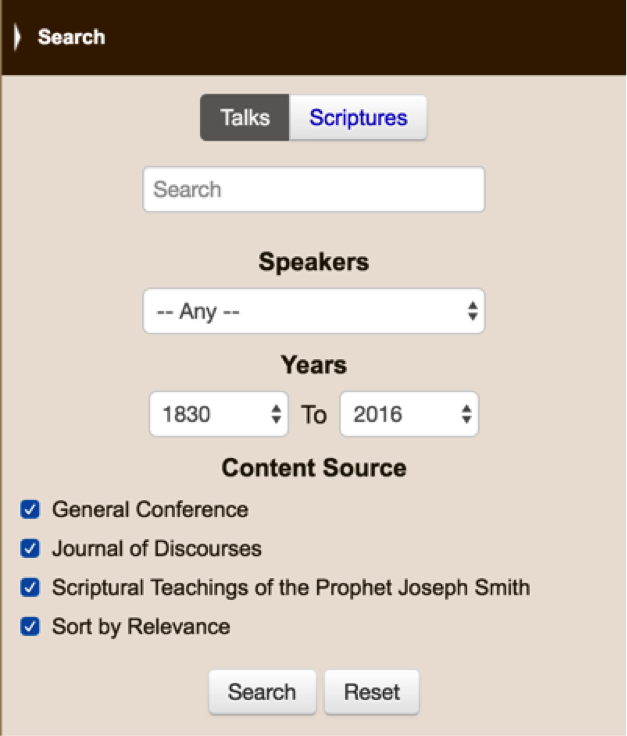
\includegraphics[width=3.5in,natwidth=310,natheight=442]{figures/sci_search.png}
		\caption[SCI \emph{TF-IDF} Search Results]{
			Samples results of a search provided to SCI Lucene search engine.
		}
	\label{fig:sci_search}
\end{figure}

Providing search capabilities is just one way \emph{LDS SCI} exposes their index. The area where \emph{LDS SCI} really shines is by its use of indexing. While an LDS discourse often has references placed in-line or at the end of the text, the reverse is not the case; LDS scriptures, including the ones found online at \url{https://www.lds.org/scriptures/}, have only footnotes. \emph{LDS SCI} has copies of LDS discourses and scriptures, indexes the references. It exposes that index in a searchable way. This allows users to reach discourses from scriptures (\url{LDS.org} does the reverse). This means that while \url{LDS.org} provides discourse-based study or scripture-only study, \emph{LDS SCI} allows for an enhanced scripture-based study, starting at verses of scripture leading to LDS discourses for potential clarification.

\emph{LDS SCI} is similar to \url{LDS.org} in that users can use them to read both scriptures and discourses. However, \emph{LDS SCI} exposes discourses pre-dating 1971, including those published in the Journal of Discourses in the 1800’s. \url{LDS.org} focuses on those published after 1971. The \emph{LDS SCI} team has already created a geographically-linked version of scriptures \url{http://scriptures.byu.edu/mapscrip/} which allows users to read scriptures (Biblical and non-biblical) and see a Google Earth view of the related area(s) on a per-chapter basis. No recommendation system exists in its interface and no index of locations is exposed directly in the user interface.

\section{Motivation}
While the \emph{LDS SCI} is helpful for the aspiring erudite of LDS content, there is currently no recommendation system for the discourses: when a user finds an interesting discourse, there is no quick, simple way to find similar/related discourse. Although the LDS website has some modern GC discourses tagged with topics, such topics are currently provided on a per-year basis only, so the discourses tagged with each topic tend to be sparse. This works when members of the LDS church want to focus on the most recent discourses only. Even with URL manipulation, attempts to expose topics for all GC discourses rather than by year do not work (\url{https://www.lds.org/general-conference/topics/2015/10} vs. \url{https://www.lds.org/general-conference/topics/})--and result in the topic index for the most recent session of GC. Sparseness for the discourses in a given topic are apparent in Figure \ref{fig:oct_2015_topics}--most topics only have 1 associated discourse and therefore have no number next to the topic’s title.

\begin{figure}[hhhhhtb]
	\centering
		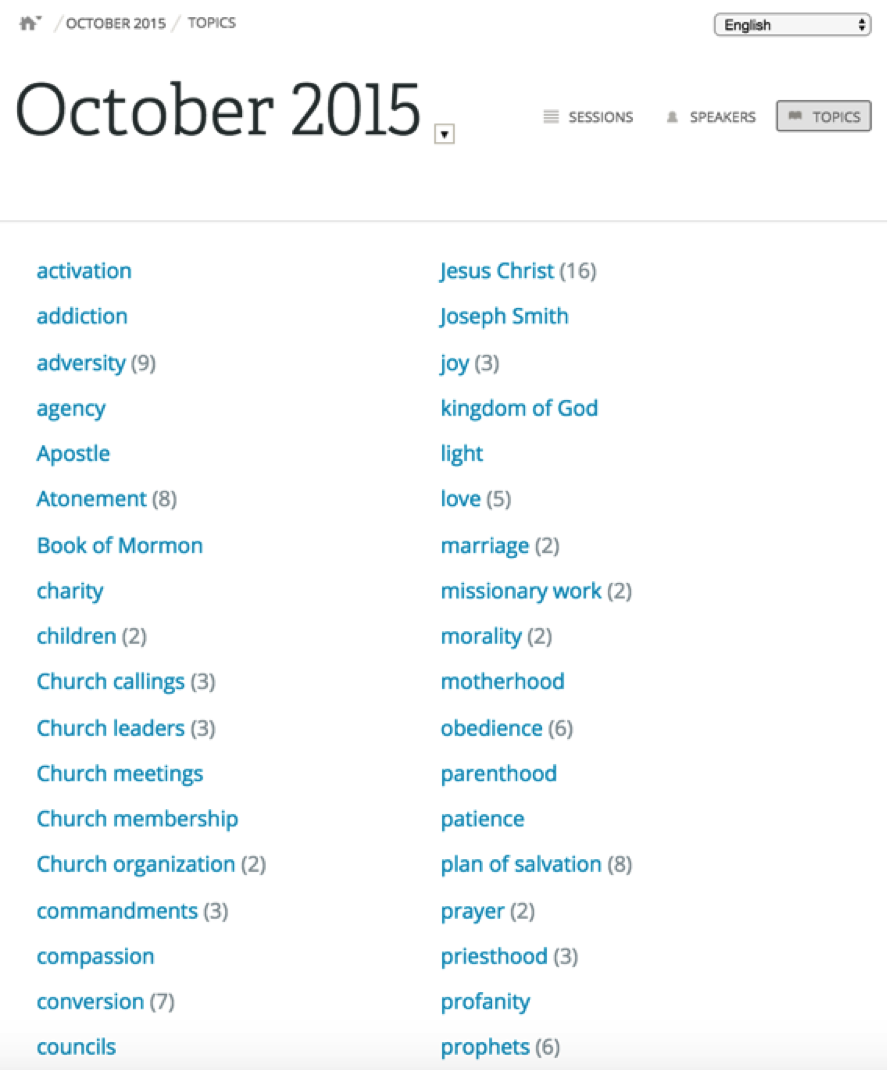
\includegraphics[width=4.5in,natwidth=410,natheight=542]{figures/oct_2015_topics.png}
		\caption[\url{LDS.org} 2015 Topics]{
			\url{LDS.org} 2015 Topics
		}
	\label{fig:oct_2015_topics}
\end{figure}

Therefore, for users of \url{LDS.org}, when a reader enjoys a particular discourse, it is difficult to locate all discourses on a given topic. It is theoretically possible to peruse every session of GC (as far back as 1971) looking for the topic in every year. The task requires a lot of clicking and will not work for discourses published before 1971 since they are not exposed online at \url{LDS.org}.

Beyond the per-year topic index provided by \url{LDS.org}, \url{LDS.org} does have a Gospel Topics index at \url{https://www.lds.org/topics/}. Under some topics, there are discourses that are selected for the topic, but they don’t promise to be results of a recommendation system that is routinely updated--and expanding the lists to see more is not possible.

\emph{LDS SCI} has discourses by topic, but was manually created and only accounts for discourses in the Journal of Discourses, which were published in the 1800’s. For those interested, digital images of the Journal of Discourses are available from the BYU online collections at \url{http://contentdm.lib.byu.edu/cdm/search/collection/JournalOfDiscourses3}.

To review, \url{LDS.org} has 2 topic indexes, one of which focuses on a per-year approach for post-1971 GC talks, the other of which appears to have been manually created. \emph{LDS SCI} has a topic index, but only for very early discourses. For a superficial study of a topic, this might be sufficient, but when one wants to reach farther than the most recent or least LDS materials--namely those in the middle--there is no search engine--and none which promises to be automatic, automatically updated, and interactive.

In the past 2 years, the query engine provided by both \url{LDS.org} and \emph{LDS SCI} have been enhanced significantly, but they still leave something to be desired: simplicity and ease of use. Dr. Liddle who built \emph{LDS SCI} has said that \emph{LDS SCI} uses a Lucene query engine, which employs a \emph{TF-IDF} search algorithm. The \url{LDS.org} engine seems to work similarly, except that it can detect phrases such as ``in talks'' and use those to automatically select to search only through discourses rather than through all LDS written materials exposed online. %[...more on how LDS SCI search engine works...]

Take for example the search query ``word of wisdom'' (without quotes in the search). This is a phrase which is more recent history of the LDS church has come to refer to a law of health. The search results look promising (shown in Figure \ref{fig:sci_results}).

\begin{figure}[hhhhhtb]
	\centering
		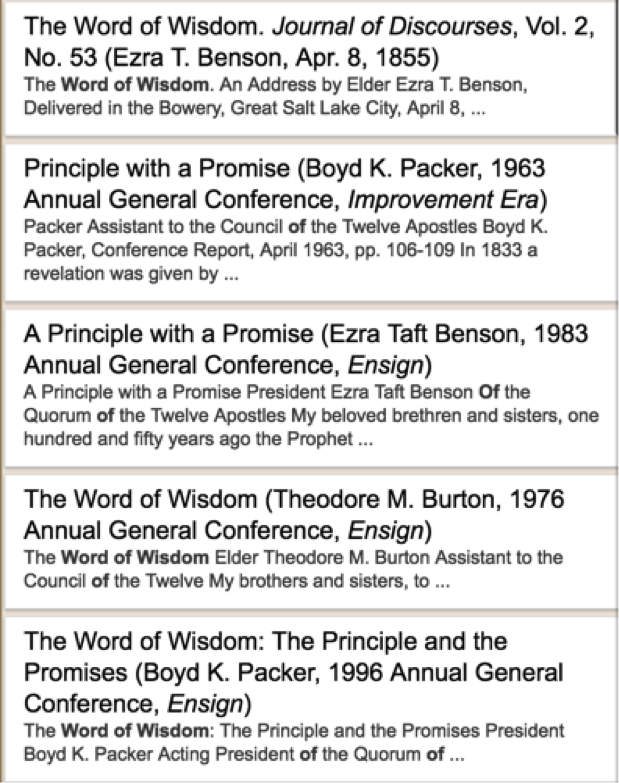
\includegraphics[width=3.5in,natwidth=310,natheight=442]{figures/sci_results.png}
		\caption[Top SCI Query Results for the search \textit{Word of Wisdom}]{

		}
	\label{fig:sci_results}
\end{figure}

But one would expect to see something by Joseph Smith Jr. to rank at the top. The confounding factor here is that ``word of wisdom'' is a modern naming convention. % TODO: Fact check this!
The word of wisdom was ``[r]evelation given through Joseph Smith the Prophet, at Kirtland, Ohio, February 27, 1833.'' (D\&C 89 Header). The earliest usage of the phrase ``word of wisdom'' in print we could find is 1873--40 years after it was revealed. (TODO: cite The Word of Wisdom—Education by President George A. Smith).

Unfortunately, without a way to determine what topics exist within all the GC discourses, there is no way for a query system to expand queries like this one. Unfortunately, even if the user does happen to find a discourse that is a pleasing match to the query, there is currently no recommendation system from that point to suggest other related discourses--just existing links and the other results for the query.

If the user were to filter to only scriptures, they would find more than 20k matches as shown in Figure \ref{fig:sci_results_20k}.

\begin{figure}[hhhhhtb]
	\centering
		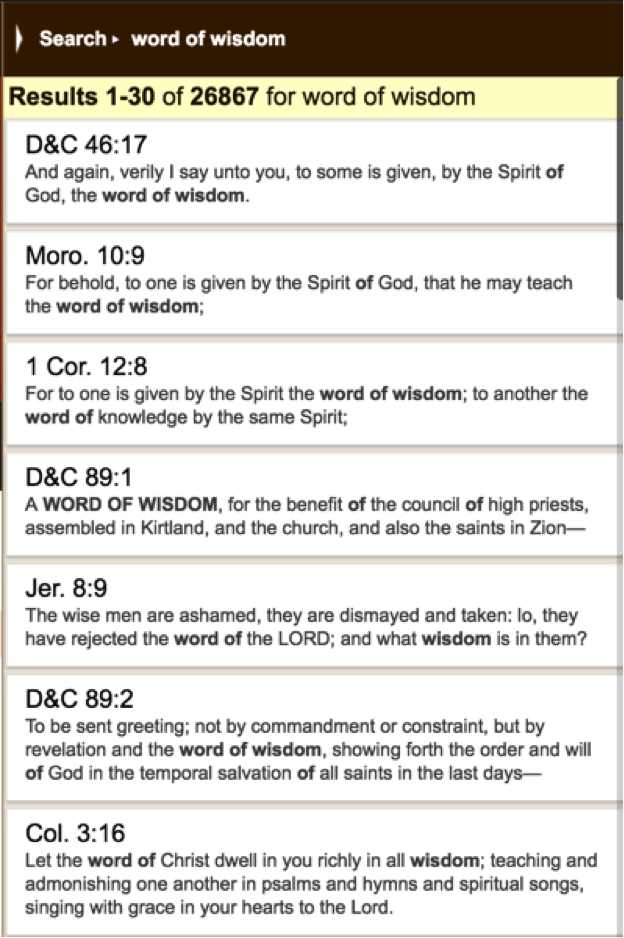
\includegraphics[width=3.5in,natwidth=310,natheight=442]{figures/sci_results_20k.png}
		\caption[20k+ SCI Results]{

		}
	\label{fig:sci_results_20k}
\end{figure}

Of those, the first one that refers to directly to a law of health is the 4th result. \url{LDS.org}, when performing the same search ranks the result referring to the law of health as the 4th result (\url{https://www.lds.org/scriptures/search?type=verse&query=word+of+wisdom}), but does so with only 39 total results. These are results that I was able to find because I understood how the search engine works. When one doesn’t know when to put quotes or doesn’t know what they are looking for, the task is more difficult, depending on the engine used. For example, when the entire query is run with quotes around it in \emph{LDS SCI}, the number of results drops from the 20k down to 7 in \emph{LDS SCI}; in \url{LDS.org}, from 39 to 8 (\url{https://www.lds.org/scriptures/search?type=verse&query="word+of+wisdom"}). Search relevance is an entire area of research and it is no wonder that companies that are able to do well in this area are able to profit from it (e.g. Microsoft with \url{https://bing.com} and Google with \url{https://google.com}). Query systems are a natural way to 'ask' a computer questions and receive results, but are obviously lacking in features.

While search query optimization would be one way to improve this area, I chose to augment the \emph{LDS SCI} toolset with recommendation features. The idea was that once a reader locates a discourse of interest, a user should be able to quickly locate similar discourses by viewing a pre-computed list of related/similar documents as a list. The list could default to displaying 5 results, but the user could interact with the list and request additional results. %There are many ways to approach this that I will explain.


\section{Recommender Systems}

One way to produce recommendations for textual data is by using post-hoc methods built on topic modeling (\citealp{blei2012probabilistic}). One well-known topic model is Latent Dirichlet Allocation, or \emph{LDA}, which is a model of word-topic assignments. From this model post-hoc algorithms extract various meta-data including probability of a topic (overall or in a document), and probability of a word in a topic. This step is fast and effective. Given a probability distribution over topics, machine learning approaches including nearest neighbor approaches (e.g. k-NN) can locate the most relevant documents. Since probability distributions are points that exist within the \emph{Probability Simplex}, or \textit{T}-space (\citealp{Krstovski2013efficient}) metrics suited for the space such as the \emph{Jensen-Shannon divergence} or the \emph{Hellinger distance} are viable metrics for determining `distance' between points. Distance is interpreted as dissimilarity (i.e. closer points are considered more similar than two distant points).

Note that topic models are not required for document recommendation. Algorithms that use token frequency and inverse document frequency, or \emph{TF-IDF}, can also be used. In such cases, documents with the similar distributions of keywords can be considered similar.

A subset of topic models aims to analyze topical trends over time. Such work includes that of \cite{hall-jurafsky-manning:2008:EMNLP} where entropy, applied on chronological disjoint sets of texts, is used as a metric of showing broadening/narrowing of topics over time. They demonstrated that the \emph{Jensen-Shannon divergence} divergence between venue \emph{venue pairings}\footnote{or disjoint sets of documents} could be used to measure level of similarity. They aptly demonstrated that topic entropy, when applied to topics on a per-year basis, could be used to describe the ebb and flow of each topic’s \emph{popularity} over time. As a result, entropy of corpora or sub-corpora can be plotted over time and compared. They demonstrated this by applying the process to entire scholarly conferences, showing that two separate conferences were converging to the have similar entropy of topics as time progressed.

In precursory work, by following the methods outlined by \cite{hall-jurafsky-manning:2008:EMNLP}, I found that the same technique could be generalized further. Instead of dividing data into venues based on conference, I divided based on gender of author, then further divided based on year of authorship. Like this work, LDA was run on this same dataset. After some trial and error, I determined that 150 was appropriate parameter setting for the number of expected topics (\citealp{bean5-LDA-ToT}).%(Bean and Ringger, 2013).
% TODO: Then why did I use 250 in this thesis???

\cite{Krstovski2013efficient} %Krstovski (2013)
show that it is possible to efficiently apply speed-up k-NN algorithms to the otherwise slow process of obtaining the nearest \emph{k} neighbors. Although they primarily tested their hypothesis using contrived datasets, it is convincing enough for us to use the same distance metric in this work. In the probability simplex where probability distributions are over topics, this the distance metric shows how similar two documents are in terms of topic content. In the k-NN algorithm, whenever two documents are close to each other in the space can be considered related or similar.

Less automated text mining on LDS religious documents includes (\citealp{hilton:2008:abinadi}) %Hilton III (2008)
. \citeauthor{hilton:2008:abinadi} aimed to discover what he calls intertextual similarity between authors of LDS-specific texts. In his work, he focused on \emph{The Book of Mormon}, although he later demonstrated that the methodology could locate results between \emph{The Holy Bible} and \emph{The Book of Mormon} (\citealp{hilton:2013:psalms}). Although topic models were not employed in his work, it may have benefited from them. Computational methods were involved, but only for portions of the process.

% TODO: Before referencing LDA, describe it or use longer name.
TODO: The following paragraph is mostly methodology and should be revised and/or moved.

Recommender systems, sometimes called recommendation systems, vary in the way that they are created. For this work, two possible systems stood out immediately for my use: LDA-based recommendation and \emph{TF-IDF} based recommendation. The latter is straightforward, easy to implement, and uses the same metrics that the query search at \emph{LDS SCI} uses. The LDA-based model brings additional features to the table, but does so indirectly. Every LDA model contains a distribution over distributions. In my case, for the model to be built, each word token is assigned to a 1 and only 1 topic. This can easily be collected and indexed, then exposed as a keyword frequency index for each topic. So on top of providing per-discourse recommendations, it could easily be used to create an index of topics, linkable to the documents with a large clustering of words in each topic! Since that was not a main focus in my work, I published the results of that at \url{http://bean5.github.io/lds-talks-by-topic/} for future use. The downside to LDA is that it is only a model. An algorithm to building the LDA model must be selected. Some algorithms include:

\begin{enumerate}
  \item Gibbs Sampling, a Markov chain Monte Carlo algorithm
  \item Variational Inference; and
  \item Expectation Maximization
\end{enumerate}

The LDA and \emph{TF-IDF} model share some similarities besides lending themselves as models for recommender algorithms. They treat each document as a bag of words. They can both be told to ignore common words, although the nature of \emph{TF-IDF} is such that high frequency words are not as noisy as they are for LDA models. `Stop-wording', a process of ignoring the words either by removal or by having code 'skip' them, nevertheless, can reduce the search space and improve algorithm time performance.

[TODO: Add more her.]

Running a Gibbs Sampler long enough is guaranteed to converge to what is called the posterior. A good initialization makes it converge sooner. Seeding with a 'good initialization' is not necessary. In previous work, I found that 1000 iterations of Gibbs converged quickly (under 1 hour) (\citealp{bean5-LDA-ToT}).
% TODO: perhaps list this: \url{https://youtu.be/UTW530-QVxo?t=1159}.

\section{Algorithms}
\begin{enumerate}
  \item k-NN
  \item ...
\end{enumerate}

\section{Metrics}
\begin{enumerate}
  \item k-NN metrics
  \item Jenson-Shannon
  \item Hellinger distance (Jenson-Shannon reduced for parallelization in k-NN; produces same results as Jenson-Shannon when used in k-NN)
\end{enumerate}

\section{LDA}
LDA stands for latent dirichlet allocation. It is a model where each token within a document is tagged with 1 and only 1 topic. Each document is treated as a bag of words.

\section{Evaluation}

Many metrics exist for the purpose of measuring \textit{goodness} of results. When ordered sets constitute the output, which is the case for search and discovery-based methods, \textit{precision} and \textit{recall} are two commonly trusted metrics. A way to balance them is to compute the F1 \textit{score} or \textit{f-measure}, which is simply the harmonic mean of the two. It is important to note that these metrics only work when a gold standard exists, e.g. when the best results are known a-priori for some test portion of the dataset. Metrics which do not require a gold standard include \textit{catalog coverage}. The \textit{serendipity} metric requires at least a baseline set of recommendations (Ge et al., 2010).

\emph{Catalog coverage} metrics show how good a system is at providing results throughout the system rather than favoring certain documents. \emph{Catalog coverage} does not require any baseline to exist. It is an intrinsic metric. \emph{Serendipity} measures how good a system is at providing results that are \textit{surprising} rather than \textit{obvious} (\citealp{Ge:2010:BAE:1864708.1864761}). \emph{Serendipity} requires a baseline to exist; it is an extrinsic metric. % I hoped to use the formulas as provided by and described by \cite{Ge:2010:BAE:1864708.1864761}, but Serendipity was not possible for use since no baseline existed.

If the two perform similarly, they will have similar output. One can measure similarity using formulas in the nDCG family (\citealp{Wang:2006:TOT:1150402.1150450}). This can lend credibility to either system if one tends to provide output that is similar to the already-accepted system. However, this is an extrinsic metric; like \emph{serendipity}, it requires the use of a \textit{common} baseline. Two systems cannot be compared to each other without the presence of a third. If they use each other as proxy as the third, he overall nDCG value for each system ends up being the same.


\section{Problems}

[TODO: Complete this section.]


\section{Open Source Tools: Docker, Mallet, npm}

\subsection{Docker\*}
Now that algorithms and metrics have been discussed, we can move on to discussing tools that can be used to create reproducible, robust, systems.

%Core to this project is the use of docker.
Dockers are Linux containers which the docker-engine (i.e. docker daemon) can build and run. They can be thought of as Linux virtual machines in some ways, although they tend to be resource/hardware agnostic since they simply share the kernel, RAM, and other hardware on the host on which they are run. They are considered lightweight since instead of running the full Linux stack for each container, only necessary files are run from within the container. This has made it easy for a new market to emerge where products that are software as a service (SaaS) can be hosted at a lower cost. Container Engine by Google (\url{https://cloud.google.com/container-engine/}) and tutum by Tutum (\url{https://www.tutum.co/}) are examples of this.

Docker has a growing community around it. In fact, Google has created an open source project called Kubernetes which aims to ``accelerate Dev and simplify Ops'' (\citealp{kube_website}). According to \cite{google_container_engine}, it is used under the covers for Container Engine, a Google cloud product. Although Linux containers have been around for some time now, the docker community has made it much more mainstream, especially for computing environments where scaling horizontally is important. Thus, companies such as Netflix and EMC find it highly beneficial. In the authors experience, Linux tools with growing communities are well backed, become robust, and tend to be both easy to use as well as empowering.

\subsection{Mallet Toolbox}
Mallet toolbox

\subsection{Node Package Manager (NPM)}
 \url{https://www.npmjs.com/}

\chapter{Methodology} \label{chp:chapter2}

/section{Overview}

I combined the methods used by \citeyearpar{hall-jurafsky-manning:2008:EMNLP} %Hall et al. (2008)
and \citeyearpar{Krstovski2013efficient} %Krstovski (2013)
to the \emph{CLDSGCT}. I then compared performance to that of an \emph{TF-IDF} model using some of the metrics outlined by \citeyearpar{Ge:2010:BAE:1864708.1864761} %Ge et al. (2010)
along with an \emph{nDCG} similarity measure. This involves comparing an LDA-based recommendation system to an off-the-shelf \emph{TF-IDF} recommendation system. Both systems will be parameterized such that they provide the top 5 recommendations for each document. I will use Collapsed Gibbs Sampling to induce parameters for an LDA (topic) model, then feed this output into a k-NN algorithm (k = 5). For k-NN’s distance metric, I will use Hellinger distance. The 5 nearest neighbors will then be sorted from nearest neighbor to farthest. This is the output that will be compared to the top 5 results for each document \emph{TF-IDF} system.

The dataset contains the same documents as those used by Mark Davies in his Corpus of LDS General Conference talks available at http://corpus.byu.edu/gc/. The authorship dates for these talks are ranges of either 1846-1886 or 1942-2013. They total over 1400 talks. Some were extemporaneously given while others were scripted. The intended audience is generally only either the male members of the church, female members of the church, or the entire church. The size and the extent of internationality of the audience is increasing over time. The LDS church currently has over 15 million members, with the majority outside the United States.

To measure the performance of \emph{RelRec}, I performed the following key tasks.

\begin{enumerate}
	\item Use \textit{Collapsed Gibbs Sampling} to infer the parameters of an LDA model;
	\item Use the Mallet toolkit will be used to run collapsed Gibbs sampling;
	\item Use k-NN with the Hellinger distance as the distance metric for \emph{RelRec}; and
	\item Use nDCG to measure similarity with a \emph{TF-IDF} system catalog coverage.
\end{enumerate}

\section{Reproducibility}
In order to be able to reproduce, share, and track work performed in the process of completing this thesis, I versioned code using git. I employed the use of both cutting edge tools as well as well-established ones. The result is code that is both highly capable and easy to follow. Ultimately, I aimed to make the code highly configurable, re-runable, measurable, and shareable.

In this section, methodology will be described, starting with code management \& organization, then tools used (programming languages, CLI tools, operating systems, libraries, databases), followed by models, algorithms \& metrics, concluding with metrics. In the \ref{fig:entire_process}, the steps (or modules) of the experiment are shown.

\begin{figure}[hhhhhtb]
	\centering
		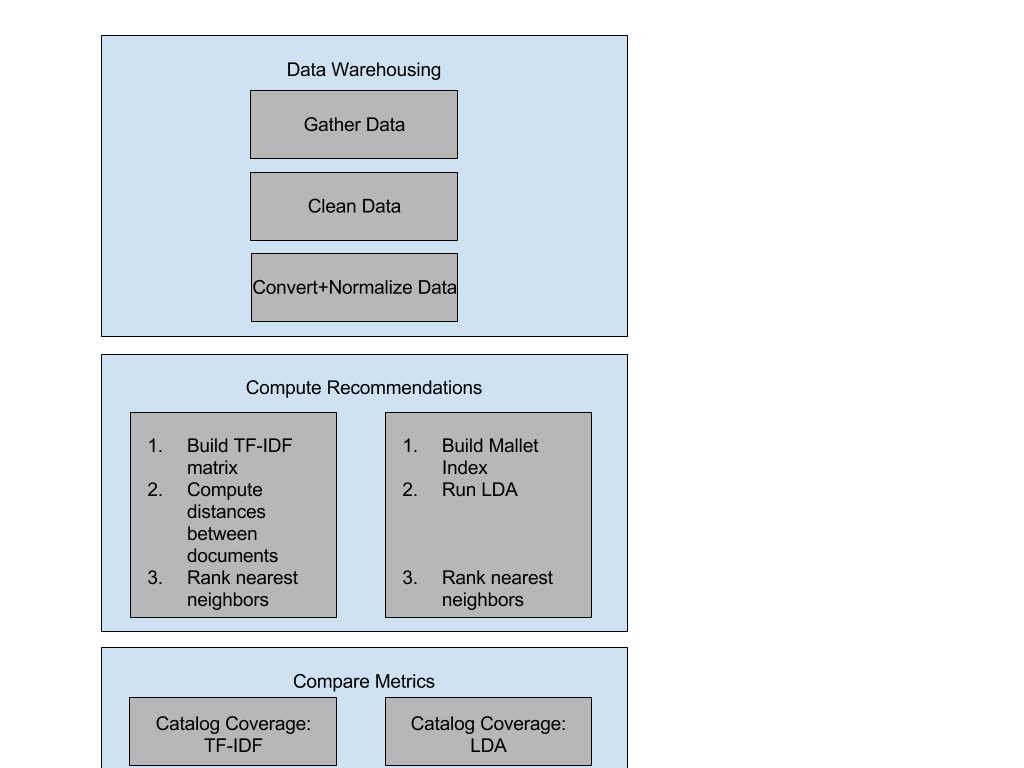
\includegraphics[width=7.5in,natwidth=810,natheight=942]{figures/entire_process.png}
		\caption[Entire Process]{
			Experiment Process\\
			The entire process for the thesis experiment outlined as `modules'. When modules are horizontally adjacent, they may be done in parallel. Note that further parallelization is possible, but not shown. Modules that are higher on the diagram are performed before lower ones.
		}
	\label{fig:entire_process}
\end{figure}

\section{Code Management + Organization}
For the experiment to be robust, it is important that it can be replicated and compared. One of the best ways to allow for this is to make the code both configurable and sharable. Thus, this section is included.

I versioned the experiment’s code in a git project along with data during the gathering process. Whenever a step completes, it outputs data which can be used as input to other modules. The code is modularized such that each docker target corresponds with a module shown previously. The docker daemon builds each target open request (as directed by make), and using docker-compose, directories are connected to the image as volumes. This allows the image to be both modular and systematic. Each docker target has a corresponding file called Dockerfile. Each Dockerfile instructs the docker daemon to obtain requisite packages, e.g. nodeJS, for the module to run the code specific to it. When the code is complete, the docker container terminates, and the next may run when Make instructs it to do so.

Viewing each docker container as a module lends to be seen as a part of the algorithm. Naturally, to each container I map an input and output folder, both located at the root of the file system. The output of multiple containers can be combined as input to subsequent ones, which was sometimes the case here. The first module’s input was actually the database graciously provided by Dr. Steven Liddle, containing pre-downloaded documents to jump-start the project.

I named each docker target logically so upon querying the docker daemon for the list of images, each image would be easy to re-run:

\begin{enumerate}
  \item obtain\_data
  \item compute\_tf\_idf\_recommendations
  \item compute\_lda\_recommendations
  \item etc.
\end{enumerate}

\subsection{Tools, Libraries, OS, Database}
I used various tools in the process of carrying for the preparation and execution of this thesis’ experiment. Table A.1 in the appendix details what they are and what they were used to do.

Core to this project was the use docker. Choosing to use docker forced me to code in all dependencies of each module either as code in the module, or as packages to be installed to each individual docker container during the docker build process. Indeed, the docker daemon builds containers by following instructions given in the files called Dockerfile. This makes each step of the experiment self-documenting. Another benefit of this is that it makes the code cloud-deployable, making it possible to easily offload work to the cloud when appropriate. Offloading to the cloud was not necessary here since I had sufficient computing resources for the project already purchased.

\subsection{Models, Algorithms \& Metrics}
Choice of algorithm \& metrics go hand-in-hand. In fact, algorithm and data can often influence each other, further influencing the selection of metrics. For example, if I were to have a gold standard or baseline of recommendation engines for the 5000+ documents used in this project, I would be able to use nDCG as a metric. Since I do not have such a baseline, such a metric cannot be used. Per xyz, I use catalog coverage, allowing the comparison of two non-baseline algorithms.

Choosing the algorithms for this project was not difficult. I selected \emph{TF-IDF}+kNN and LDA+kNN as my main topic-modeling algorithms. \emph{TF-IDF} is straight-forward to understand and code. LDA is more difficult to code and is actually a topic model. Luckily, open source projects exist where an algorithm is already provided, which I quickly opted to use.

Given that I had prior experience using Gibbs Sampling to generate LDA models ([TODO: Cite here.]) using the open source mallet toolkit ([TODO: cite here]), the choice to select that was logistical (optimizing to let me have time to spend on other areas of this work). EM lends itself to parallelization, but on my dataset, I knew that Gibbs Sampling would only take about 10 minutes to run, which is not an issue. The cost-benefit of changing algorithms was too high, at least when it comes to building the LDA model via parallelized algorithm. In my case, I used the mallet toolbox ([TODO: cite in introduction]) which provides the Gibbs Sampling algorithm to estimate the LDA model.

% TODO: Double check whether Jenson-Shannon was used (check prospectus).
% TODO: Add more algorithm notes here and move this table to a better location.
% TODO: 'core module' is a new term introduced here!
\begin{center}
	\begin{tabular}[pos]{| l | l | l | l | l | l |}
		\hline
		Algorithm & Variable Name & Variable Type & Input Value & Use & Reason \\ \hline

		k-NN & k & integer & 100 & Sets number of neighbors to \\ return for each document. & Using a value of 100 requires more computing, but also allows us to compare the models for up to 100 recommendations per document. \\ \hline

		Gibbs Sampling & t & integer & 250 & Sets number of topics to find & In previous research I determined that 250 was a good number for this variable. \\ \hline

		k-NN distance metric \\
		for \emph{TF-IDF} model & distance & function & Cosine & Distance metric allows algorithm to measure distance between documents in the model. & Intuitive and well-known. Others functions exist for this, but are left to future work to use. \\ \hline

		k-NN distance metric \\
		for LDA model & distance & function & Jenson-Shannon & Distance metric allows algorithm to measure distance between documents in the model. & Well-known and works for vectors in the probability simplex. \\ \hline

		\emph{TF-IDF} & stop words & list of word strings & none & Sets words to ignore in model. & Assigns words a value of 0 TF and 0 IDF values or removes them altogether to shrink vector space and accelerate computing (depends on actual algorithm implementation). \emph{TF-IDF} is robust against high-frequency words since they automatically receive low TF and low IDF values. \\ \hline

		Preparing input LDA & stop words & list of word strings & default mallet list + handful of religious words [TODO: which words?] & Removes stopwords at indexing time (module x [TODO: name exact module here]). & LDA is not super robust against common words. \\ \hline
		normalization & to\_lower\_case & boolean & true & If true, tells algorithm to lowercase all text. & To allow all following algorithms to ignore case, the simplest way to do so was to lowercase everything before completing the data preparation core module. \\ \hline
	\end{tabular}
\end{center}

% TODO: cite instead of link?
The core of this project came down to organization, good testing (to ensure bug-free code), and study of any tools that would end up being helpful in processing. kNN is a machine learning algorithm which as input requires the value for k and a selection of a distance metric. The output of \emph{TF-IDF} and LDA are both in vectors, but LDA’s vectors lay within the probability simplex. Distance metrics had to be appropriate for the space. For \emph{TF-IDF} vectors, I opted to use cosine similarity; for LDA, Jensen-Shannon (\url{https://en.wikipedia.org/wiki/Jensen%E2%80%93Shannon_divergence, http://maroo.cs.umass.edu/pub/web/getpdf.php?id=1101}). % TODO: (or was it Hellinger? \url{https://www.quora.com/How-can-I-compute-the-Hellinger-distance-between-documents-based-on-topic-proportions-generated-by-Latent-Dirichlet-Allocation}).

To evaluate the recommendations provided as output from the ordered kNN results, a common metric had to be employed. I chose to measure the goodness of each set using the catalog coverage metric. % TODO: remove passive voice here.

For reproducibility, the following table shows the values, settings, and configurations selected for the algorithms.

By using the aforementioned metrics, this study aims to prove the following hypothesis
	\begin{quote}
		$H_{1}:$ \emph{RelRec} will provide better coverage than a \emph{TF-IDF} system.

		%$H_{2}:$ \emph{RelRec} is more intuitive than emph recommendation systems since it has greater ability to disambiguate word sense by topic.
	\end{quote}

%\chapter{Results \& Evaluation} \label{chp:chapter3}

[TODO: insert here: samples of topics: a sanity check]

[TODO: insert here: samples of TF-IDF words]

[TODO: insert here: display graph of results]

\begin{figure}[hhhhhtb]
	\centering
		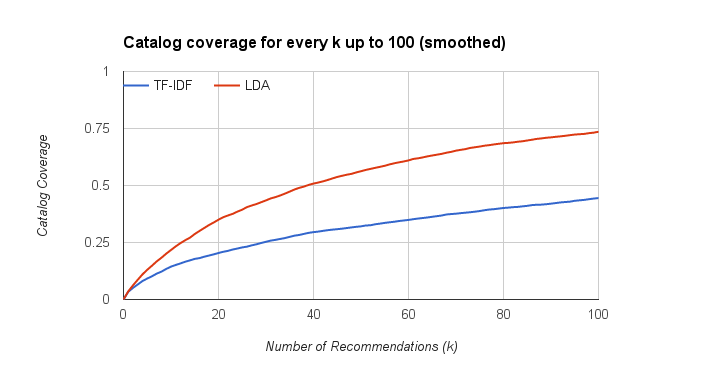
\includegraphics[width=5.5in,natwidth=510,natheight=642]{figures/catalog_coverage_0_100.png}
		\caption[Catalog Coverage Values for All Models]{
			Catalog Coverage Values for All Models
		}
	\label{fig:catalog_coverage_0_100}
\end{figure}

[TODO: insert here: display some topics here, put full list of topics in appendix?]

%\include{chapter4_conclusion}
%\include{chapter5_future_work}




%%%%%%%%%%%%% begin Bibliography %%%%%%%%%%%%%%%%%
\phantomsection %Forces a new section prior to setting the bibliography reference point
\bibliographystyle{IEEEtran}
\addcontentsline{toc}{chapter}{Bibliography}
\bibliography{refs}

% Bibliographies are best created and maintained using BibTeX
% To use Bibtex, create a bibliography file, e.g., refs.bib
% The sample file sources.bib shows examples of different
% bibliographic entries.
% The bibliography is created by executing:
%  1.  latex, 2. bibtex, 3. latex, 4. latex
%%%%%%%%%%%%%%%% end Bibliography %%%%%%%%%%%%%%%%%

%Included because WinEdit is RETARDED and it needs it for Gather Purposes:
%input "refs.bib"


% Include appendix sections here:
% each appendix should be a file with a .tex extension and the text
% of the file should begin with \appendix{Appendix Title}, followed
% by the contents of the appendix
\appendix{Sample Appendix}

\section{Width Based on Page Size Figure Example} \label{sec:appendxia_figure_example}
Here's an example of a figure whose width depends on the width
of the page. You can see if as Figure \ref{fig:appendix_some_pic}.

\begin{figure}[htbp]
  \centering
  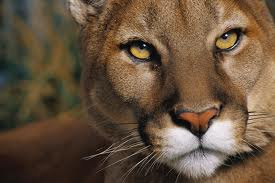
\includegraphics[width=0.45\textwidth]{figures/appendixa/some_pic}
  \caption[Example Width Based on Page Size Figure]{
    This is an example of a figure whose width will be 45\% of the
    width of the page. If you'd like to see a figure with a fixed
    width then you can see it as Figure \ref{fig:intro_stuff} in
    Section \ref{sec:intro_figure_example}. Just FYI, I made this
    figure with PowerPoint and then copied it and pasted it into
    wmf2eps and choose the "Paste EMF" option. It will generate
    a larger file, but it will look a TON better than the
    "Paste WMF" option and the "Paste DIB" option will paste the
    rasterized image that won't scale well at all.}
  \label{fig:appendix_some_pic}
\end{figure}

%End the document
\end{document}
